\documentclass[a4paper,hidelinks,14pt]{extarticle}

\usepackage[utf8]{inputenc}
\usepackage[T2A]{fontenc}
\usepackage[english, russian]{babel}
\usepackage{lipsum}
\usepackage{amsmath}
\usepackage{amssymb}
\usepackage{amsfonts}
\usepackage{mathtools}
\usepackage{datetime}
\usepackage[pdftex]{graphicx}
\usepackage{indentfirst}
\usepackage{asymptote}
\usepackage{systeme}
\usepackage[dvipsnames]{xcolor}
\usepackage{lastpage}
\usepackage{fancybox,fancyhdr}
\usepackage{hyperref}
\usepackage[framed]{matlab-prettifier}
\usepackage	{pythonhighlight}
\usepackage[font={small,it}]{caption}
\fancyhead[L]{Лабораторная работа №5}
\fancyhead[C]{}
\fancyhead[R]{\textit{Связь непрерывного и дискретного}}
\fancyfoot[L]{}
\fancyfoot[C]{Страница \thepage\space из \pageref{LastPage}}
\fancyfoot[R]{}
\pagestyle{fancy}

\begin{document}
	\begin{titlepage}
		\setlength{\parindent}{0ex}
		
		\begin{center}
			\textsc{
				\vspace{1ex}
				Научно исследовательский университет ИТМО \\
				\vspace{0.5ex}
				Факультет систем управления и робототехники \\
				\vspace{0.5ex}
			}
		\end{center}
		
		\vspace{50mm}
		
		\begin{center}
			Отчет по лабораторной работе №5 \\
			Связь непрерывного и дискретного
		\end{center}
		
		\vspace{50mm}
		
		\begin{minipage}{.55\linewidth}
			Выполнил студент группы R3280
			
			Преподаватели
		\end{minipage}
		\hfill
		\begin{minipage}{.5\linewidth}
			\begin{flushright}
				Мовчан И. Е.
				\\
				Пашенко А.В., Перегудин А. А.
			\end{flushright}
		\end{minipage}
		
		\vfill
		\begin{center}
			Санкт-Петербург
			\\
			2024
		\end{center}
		
	\end{titlepage}
	
	\section{Непрерывный и дискретный Фурье}
	Рассмотрим прямоугольную фунцию П $: \mathbb{R} \rightarrow \mathbb{R}$:
	$$
		\text{П}(t) =
		\begin{cases*}
			1, \ |t| \leq \frac{1}{2} \\
			0, \ |t| > \frac{1}{2}
		\end{cases*}	
	$$
		
	
	\subsection{Истинный Фурье-образ}
	
	Найдём аналитическое выражение для Фурье-образа функции П:
	$$
	\hat{\text{П}}(\nu) = \int \limits_{-\infty}^{+\infty} \text{П}(t) e^{-2\pi i \nu t} dt = \int \limits_{-1/2}^{1/2} e^{-2\pi i \nu t} dt = \frac{i e^{-2\pi i \nu t}}{2 \pi \nu} \bigg|_{-1/2}^{1/2} = \frac{\sin(\pi \nu)}{\pi \nu}
	$$
	
	Используя найденное выражение, построим графики функций П$(t)$ и $\hat{\text{П}}(\nu)$:
	\begin{figure}[h]
		\centering
		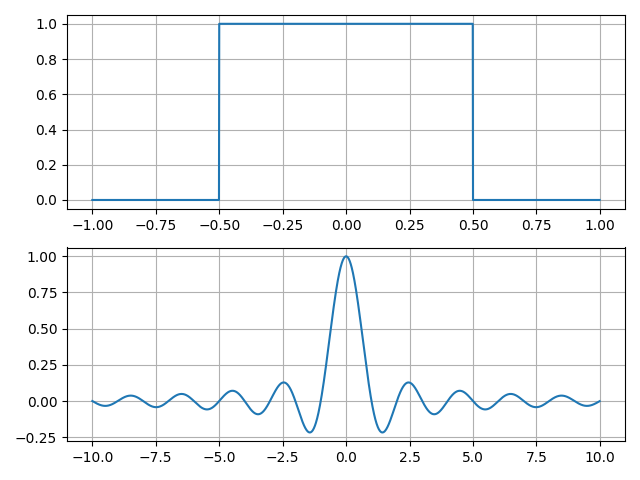
\includegraphics[scale=0.7]{./images/1.png}
		\caption{Графики функций П$(t)$ и $\hat{\text{П}}(\nu)$}
	\end{figure}
	
	Данный результат уже был нам известен, так что не будем заострять на нём какое-то особое внимание.
	
	\subsection{Численное интегрирование}
	
	Воспользуемся теперь численным интегрированием и найдём образ Фурье и саму функцию с его помощью. Итак, как и прежде, нам необходимо посчитать интегралы (только теперь программными средствами), а потому задействуем Python. Код представлен ниже:
	\begin{python}
t = np.linspace(-1, 1, 10**3)
v = np.linspace(-5, 5, 10**3)

num_fourier = np.array([])
for i in v:
	num_fourier = np.append(num_fourier, [np.trapz(y*np.exp(-2*np.pi*1j*i*t), t)])
		
num_y = np.array([])
for i in t:
	num_y = np.append(num_y, [np.trapz(num_fourier*np.exp(2*np.pi*1j*i*v), v)])
	\end{python}
	
	Графики тогда будут выглядеть следующим образом:
	
	\begin{figure}[h]
		\centering
		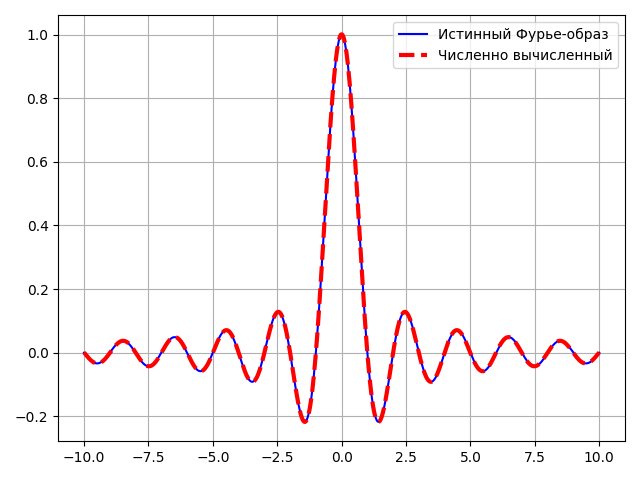
\includegraphics[scale=0.7]{./images/2.png}
		\caption{График Фурье-образа количество точек $k=10^3$}
	\end{figure}
	
	\begin{figure}[h]
		\centering
		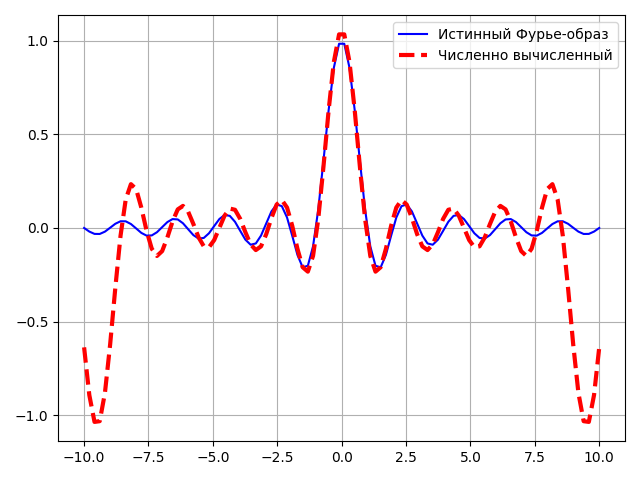
\includegraphics[scale=0.7]{./images/2_1.png}
		\caption{График Фурье-образа количество точек $k=20$}
	\end{figure}	
	
	Как можно видеть, чем мельче шаг интегрирования, тем более близки мы становимся к истинному значению Фурье-образа функции.
	
	Это же касается и восстановленной функции, только там появляется ещё один важный параметр - промежуток интегрирования по $[-\nu_0, \nu_0]$, чем он, соответственно, большой точности мы достигаем при восстановлении самой функции. Это можно видеть на рисунках \ref{3} и \ref{4}.
	
	Также стоит отметить, что используемый метод весьма медлителен - даже не при самых больших промежутках и не при самом маленьком шаге мы вынуждены ждать по 10 и более секунд, чтобы получить хоть какие-то результаты...
	
	\subsection{Использование DFT}
	
	Решить проблему с быстродействием помогает \textit{быстрое преобразование Фурье} (БПФ или fft). Проверим его в действии, написав в всего строчки (отметим также, что мы сделали наше преобразование \textit{унитарным}, прописав в качестве аргумента norm="ortho"):
	
	\begin{python}
num_fourier_f = np.fft.fftshift(np.fft.fft(y, norm="ortho"))
num_y_f = np.fft.ifft(np.fft.ifftshift(num_fourier_f), norm="ortho")
	\end{python}
	
	Графики для данного метода нахождения преобразования представлены на рисунках \ref{5} и \ref{6}.
	
	
	\begin{figure}
		\centering
		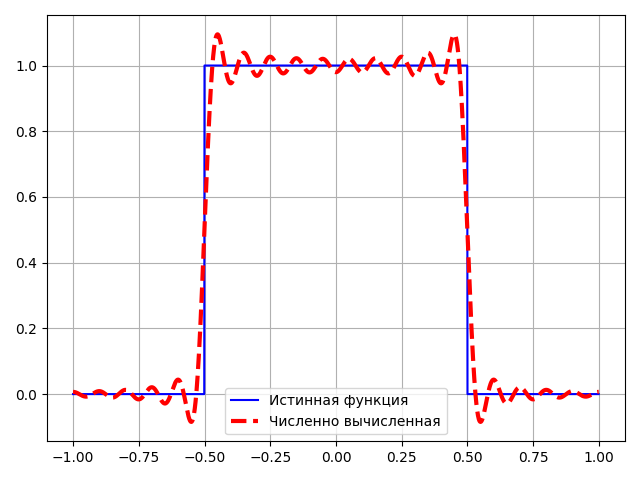
\includegraphics[scale=0.7]{./images/3.png}
		\caption{Графики функций при количество точек $k=10^3$ и $\nu_0=10$}
		\label{3}
	\end{figure}
	
	\begin{figure}
		\centering
		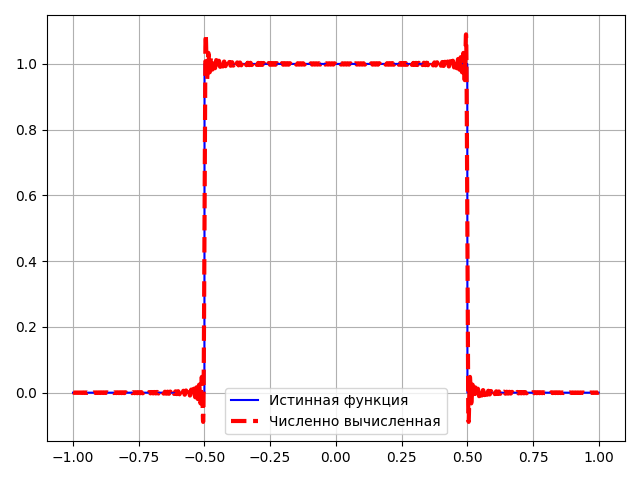
\includegraphics[scale=0.7]{./images/3_1.png}
		\caption{Графики функций при количество точек $k=10^3$ и $\nu_0=100$}
		\label{4}
	\end{figure}
	
	\begin{figure}
		\centering
		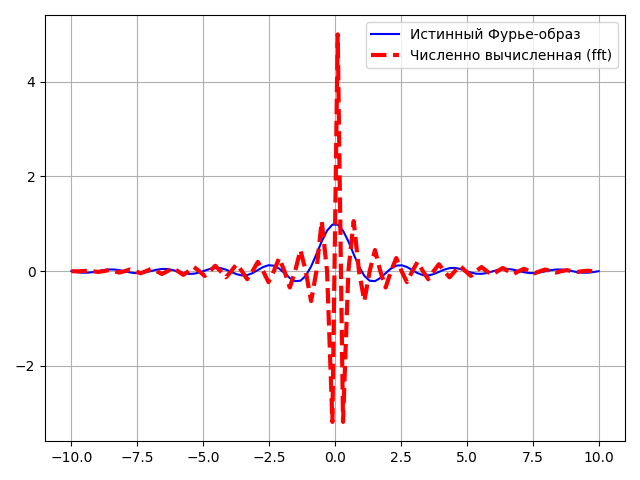
\includegraphics[scale=0.7]{./images/4.png}
		\caption{График Фурье-образа для fft}
		\label{5}
	\end{figure}
	
	\begin{figure}
		\centering
		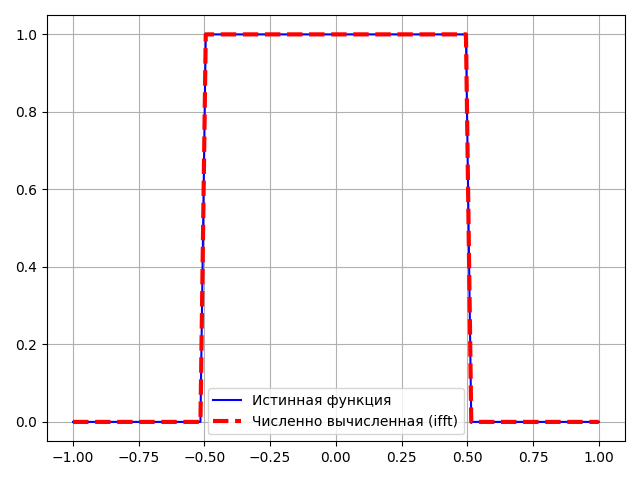
\includegraphics[scale=0.7]{./images/5.png}
		\caption{Графики функций для fft}
		\label{6}
	\end{figure}
	
	Можно видеть, что наша функция восстановилась чуть ли не \textit{идеально}, а вот Фурье-образ мало напоминает нам об истинной его сущности.
	
	\subsection{Объяснения}
	Всё дело в том, что fft хоть и работает быстро, но строит Фурье-образ для \textit{дискретного} случая, поэтому-то и восстановление является практически идеальным (ведь мы по сути восстанавливаем исходные значения, а не саму функцию). Однако у этого есть и недостаток: мы получаем Фурье-образ не нашей функции, а её дисретного аналога; именно поэтому он мало чем похож на истинный Фурье-образ исходного сигнала.
	
	Если же мы будем рассматривать метод, использующий численное интегрирование, то мы увидим ровно противоположную ситуацию: Фурье-образ достаточно близко к исходному, однако восстановление работает не так хорошо, и мы получаем более-менее правдоподобный результат только при больших промежутках и маленьких шагах (и то, получающаяся функция терпит разрыв в точках не непрерывности), то есть когда вычисления являются достаточно трудоёмкими.
	
	\subsection{Приближение непрерывного с помощью DFT}
	
	Преимущества обоих методов (точность в случае численного интегрирования с помощью trapz и быстродействие в случае fft) можно совместить и получить метод, дающий правильный Фурье-образ за достаточно короткое время. Для этого воспользуемся...
	
	
	
\end{document}